\documentclass{standalone}
\usepackage{tikz,amssymb}
\usetikzlibrary{
	patterns,
	shapes,
	arrows,
	positioning,
	decorations.markings,
	decorations.pathmorphing,
	circuits.logic.US,
	circuits.logic.IEC,
	fit,
	calc,
	plotmarks,
	matrix
}

\tikzset{
%Define standard arrow tip
>=stealth',
%Define style for different line styles
help lines/.style={dashed, thick},
axis/.style={<->},
important line/.style={thick},
connection/.style={thick, dotted},
punkt/.style={
rectangle,
rounded corners,
draw=black, thick,
text width=4.5em,
minimum height=2em,
text centered,
},
pil/.style={
->,
very thick,
shorten >=2pt},
pilr/.style={
<-,
very thick,
shorten <=2pt}
}

\begin{document}

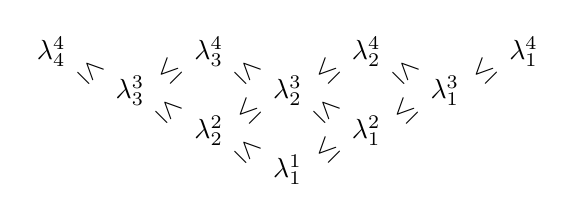
\begin{tikzpicture}
[scale=1, thick]
\def\ve{.5}
\node at (-1,\ve) {$\lambda^4_4$};
\node at (1,\ve) {$\lambda^4_3$};
\node at (3,\ve) {$\lambda^4_2$};
\node at (5,\ve) {$\lambda^4_1$};
\node at (0,0) {$\lambda^3_3$};
\node at (2,0) {$\lambda^3_2$};
\node at (4,0) {$\lambda^3_1$};
\node at (1,-\ve) {$\lambda^2_2$};
\node at (3,-\ve) {$\lambda^2_1$};
\node at (2,-2*\ve) {$\lambda^1_1$};
\node[rotate=-45] at (1.5,-1.5*\ve) {$\le$};
\node[rotate=-45] at (.5,-.5*\ve) {$\le$};
\node[rotate=-45] at (2.5,-.5*\ve) {$\le$};
\node[rotate=45] at (3.5,-.5*\ve) {$\le$};
\node[rotate=45] at (1.5,-.5*\ve) {$\le$};
\node[rotate=45] at (2.5,-1.5*\ve) {$\le$};
\node[rotate=45] at (2.5,.5*\ve) {$\le$};
\node[rotate=45] at (4.5,.5*\ve) {$\le$};
\node[rotate=45] at (.5,.5*\ve) {$\le$};
\node[rotate=-45] at (1.5,.5*\ve) {$\le$};
\node[rotate=-45] at (3.5,.5*\ve) {$\le$};
\node[rotate=-45] at (-.5,.5*\ve) {$\le$};
\end{tikzpicture}
















\end{document}
